\section{Convolutional Neural Networks}  

  With convolutions in mind, we 

\subsection{Convolution Arithmetic} 

\subsection{Pooling Layers}  

  What we eventually hope for is that we can extract higher level features that can be encoded in moderate-dimensional vectors. Unfortunately, the rate at which regular convolutional filters (especially when there is padding and a stride of $1$) does not shrink the resolution of the input images at a fast enough rate. For example, having a $3 \times 3 \times 3 \times 3$ kernel with no padding on a $(3, 100, 100)$ image will decrease the dimensions to only $(3, 98, 98)$ only. Therefore, we do some very simple operations to reduce the resolution faster. 

  \begin{figure}[H]
    \centering 
    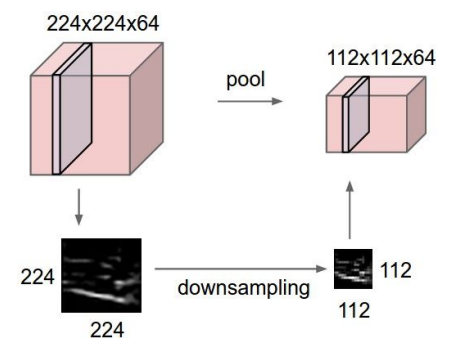
\includegraphics[scale=0.4]{img/max_pool1.png}
    \caption{} 
    \label{fig:max_pool1}
  \end{figure}

  \begin{figure}[H]
    \centering 
    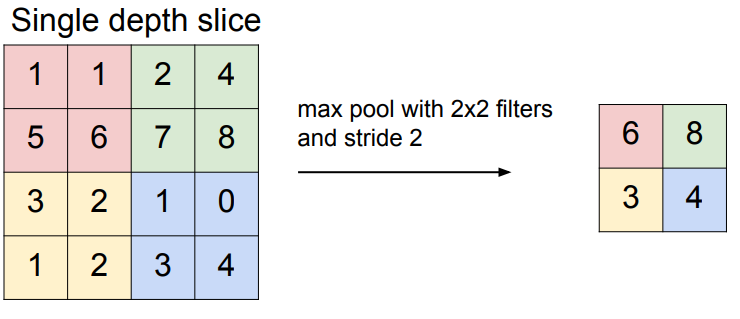
\includegraphics[scale=0.4]{img/max_pool2.png}
    \caption{} 
    \label{fig:max_pool2}
  \end{figure}

  \begin{definition}[Pooling Layers]
    A pooling layer takes in an input image of dimension $(C, H, W)$ and essentially does \textbf{downsampling} on it, involving some method of pooling local groups of pixels together into one value. There are several ways to do this: 
    \begin{enumerate}
      \item \textbf{Max Pooling} refers to dividing each channel of the image into a ``checkerboard" of $P \times P$ (where $P$ is a hyperparameter and does not necessarily have to be a square) matrices and simply choosing the maximum pixel value from it. 
      \item \textbf{Average Pooling} is the same as max pooling but we just take the average. 
    \end{enumerate}
    Clearly, these are not expensive operations and are an effective way to downsample. Therefore, the same $(3, 100, 100)$ image, after one convolutional layer followed by a pooling layer, will result in a $(3, 49, 49)$ image.  
  \end{definition}

  Ultimately, after a series of convolutions and pooling, we would want to reduce this image to a form of $(C, H, W)$, where both $H$ and $W$ are small and $C$ is large. This is because for each value of $C$, say $C = 1$, the cross section $\{(1, W, H)\}$ would encode the value of the feature identified by $C$. In fact, it could be the fact that both $H$ and $W$ are $1$, and $C = 10$. Then, we would essentially be looking at an array of $10$ numbers, which could encode the presence of some abstract features. For example, the first value $C = 1$ would encode the presence of an eye, which in the end has a value of $0.9$ (high probability), the second $C = 2$ could encode the presence of an ear, and so on. 

\subsection{Architecture} 

  Perhaps the sparsity of these maps may not allow the convolutional layers alone to extract all the features we need, so it is common to unwrap the features and then add a few fully connected layers at the end, which is much more computationally feasible now that the convolutions and pooling layers have reduced the dimensionality whilst extracting useful features with the concept of locality. This turns out to have comparable performance to regular MLPs with a fraction of the computational cost, and can easily reach $98\%$ validation accuracy on the MNIST dataset. 

  \begin{center}
    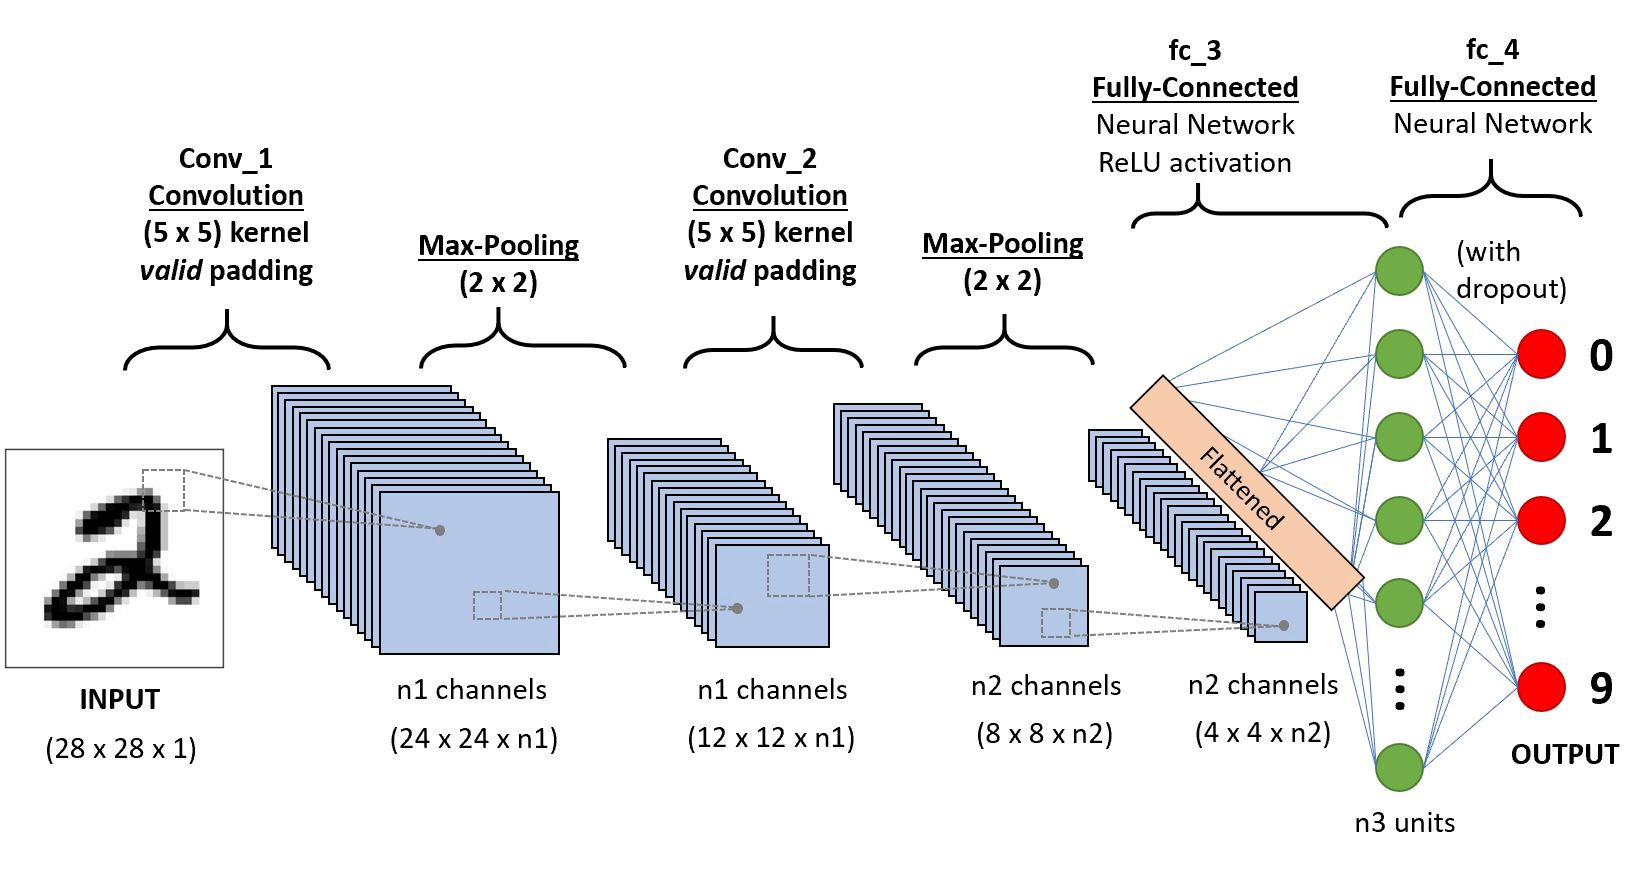
\includegraphics[scale=0.25]{img/CNN_architecture.jpeg}
  \end{center}

\subsection{Backpropagation}

  The fully connected layers are all taken care of, but now it's the convolutional layers and the pooling layers. The convolutional layers are also linear maps, so they can be treated the same way. However, the pooling layers may be nonlinear. 
  \begin{enumerate}
    \item Average pooling is linear, so no worries here. 
    \item Max pooling is not linear, but it is the next best thing: piecewise linear. 
  \end{enumerate}

